\documentclass[12pt]{extarticle}
\usepackage[margin=1in]{geometry}
\usepackage{amsmath}
\usepackage{url}
\usepackage{color}
\usepackage{graphicx}

% my commands
\newcommand{\R}{\mathbf{R}} % walker
\newcommand{\ket}[1]{\left| #1 \right>}
\newcommand{\bra}[1]{\left< #1 \right|}
\newcommand{\braket}[2]{\left< #1 | #2 \right>}

\title{Report on Research Rotation I}
\author{Cody L. Petrie}

\begin{document}
\maketitle

\abstract{I have learned how to use Variational Monte Carlo (VMC) and Diffusion Monte Carlo (DMC) methods to solve the Schr\"odinger equation for simple systems. I have applied these methods to both 1D and 3D harmonic oscillators, as well as systems with $x^4$ potentials. I was able to verify that my results agreed with the exact results for the harmonic oscillator systems. I have learned the basics of Auxiliary Field Diffusion Monte Carlo (AFDMC) and have described the additions that I plan to make to the existing AFDMC code.}

% include sections here
\section*{Introduction}
Solving the Schr\"odinger equation for many-body nuclear systems gets difficult as the number of particles increases and as the potential term in the Hamiltonian gets more complicated. To overcome this we can use Monte Carlo methods. These methods require a good nuclear Hamiltonian and a good trial wave function. One of the things that makes it difficult to get a good nuclear Hamiltonian is the spin dependance. Another thing that makes them difficult to obtain is the little understanding that we have of the strong nuclear force, which is responsible for the binding together of quarks to form nucleons as well as binding nucleons together to form nuclei. Since we cannot come up with exact expressions for these strong force interactions we use phenomenological methods to obtain the potentials. The usual Hamiltonians come from the Argonne and Urbana potentials \cite{wiringa1984, muller1981}. The Hamiltonians that we use are of the form
\begin{equation}
  H=\sum\limits_{i=1}^{A} \frac{\mathbf{p}^2}{2m} + V,
\end{equation}
where $V$ takes the form
\begin{equation}
  V = \sum\limits_{i<j}^{A} \sum\limits_{p} v_{p}(r_{ij}) \mathcal{O}^{(p)}_{ij}.
\end{equation}
For our purposes $p$ will run from $1-6$ and the $\mathcal{O}^{(p)}$ are given by 1, $\mathbf{\sigma}_i \cdot \mathbf{\sigma}_j$, $3\mathbf{\sigma}_i \cdot \hat{r}_{ij}\mathbf{\sigma}_j \cdot \hat{r}_{ij} - \mathbf{\sigma}_i \cdot \mathbf{\sigma}_j$, and the same things multiplied by $\mathbf{\tau}_i \cdot \mathbf{\tau}_j$. More detail can be found in \cite{schmidt1999}. This Hamiltonian is then used in the Schr\"odinger equation
\begin{equation}
  i\frac{\partial \Psi(R,S,t)}{\partial t} = H\Psi(R,S,t)
\end{equation}
to solve for the ground state energy and wavefunction for particular nuclear systems. The two nuclear systems that we typically study are atomic nuclei and nuclear matter.

In preparation for using and modifying the current Auxiliary Field Diffusion Monte Carlo (AFDMC) code \cite{schmidt1999,gandolfi2014} I have used Variational Monte Carlo (VMC) and Diffusion Monte Carlo (DMC) as described in \cite{foulkes2001,kosztin1996} to solve the quantum harmonic oscillator(QHO) and the similar problem with an $x^4$ potential. I will first describe these two Monte Carlo methods in a general form, and then I will apply the DMC method to the QHO.




\section*{Variational Monte Carlo}
There are many good books that describe the basics of the VMC method, but I found the explanation in \cite{foulkes2001} to be particularly useful, and I have drawn heavily from this paper to build my understanding of VMC and DMC.
\subsubsection*{Monte Carlo Integration}
Before explaining variational Monte Carlo (VMC) I am going to describe the method for performing Monte Carlo integration. Assume that we are trying to integrate the function
\begin{equation}
  I = \int g(\R)d\R.
\end{equation}
This can be rewritten as
\begin{equation}
  I = \int f(\R)P(\R)d\R
\end{equation}
where $f(\R)=g(\R)/P(\R)$, and $P(\R)$ is the importance function (probability density). In our case $P(\R)$ can be interpreted as $\left<\psi_T|\psi_T\right>$ where $\left|\psi_T\right>$ is the trial wave function. Also note that $\R=(\mathbf{r}_1, \mathbf{r}_2, \ldots, \mathbf{r}_n)$, where $\mathbf{r}_i$ is the position of the ith particle, and a specific $\R$ is called a {\it walker}. Now you say that the integral looks like the expectation value of the random variable $f(\R)$ (Think of $\left< \hat{H} \right> = \int_{-\infty}^{\infty} \left<\psi\right|\hat{H}\left|\psi\right>$).

Now the integral can be determined by drawing an infinite number of samples from $f(\R)$ and computing the average.
\begin{equation}
  I = \lim_{N \to \infty} \frac{1}{N}\sum\limits_{n=1}^N f(\R_n)
\end{equation}
The integral can then be approximated by
\begin{equation}
  I \approx \frac{1}{N} \sum\limits_{n=1}^N f(\R_n).
\end{equation}
Notice that by the central limit theorem if $f(\R)$ has mean $\mu$ and standard deviation $\sigma^2$ then $I$ will have mean $\mu$ and standard deviation $\sigma/\sqrt{N}$.

\subsubsection*{The Metropolis Algorithm}
Often times sampling from the distribution $P(\R)$ is difficult because $P(\R)$ is complicated and difficult to invert. The metropolis algorithm allows us to sample complicated $P(\R)$'s. The steps are as follows.
\begin{enumerate}
  \item Start at some random walker $\R$.
  \item Propose a move to a new position $\R'$, pulled for a distribution $T(\mathbf{R \leftarrow R'})$.
  \item The probability of accepting the move is given by
    \begin{equation}
      A(\mathbf{R' \leftarrow R}) = \mathrm{min}\left( 1, \frac{T(\mathbf{R' \leftarrow R}) P(\R'))}{T(\mathbf{R' \leftarrow R}) P(\R))} \right).
    \end{equation}
    $T(\mathbf{R' \leftarrow R})$ can be 1 or a Gaussian centered around the current walker, or something else entirely. A random number is then pulled from $r=U(0,1)$, and the move is accepted if $r<A(\mathbf{R' \leftarrow R})$.
  \item Repeat from step 2.
\end{enumerate}

\subsubsection*{VMC}
To do VMC you first start with a trail wave function $\Psi_T$. The accuracy of VMC is sensitive to the choice of $\Psi_T$. The trial wave function is then used to find a rigid upper bound on the ground state energy, $E_0$.
\begin{equation}
  E_V = \frac{\int \Psi_T^*(\R)\hat{H}\Psi_T(\R)d\R}{\int \Psi_T^*(\R)\Psi_T(\R)d\R} \le E_0
\end{equation}
The methods above are used to evaluate this integral which can be written as
\begin{equation}
  E_V = \frac{\int |\Psi_T(\R)|^2 [\Psi_T^{-1}(\R)\hat{H}\Psi_T(\R)d\R]}{\int |\Psi_T(\R)|^2 d\R}.
\end{equation}
Random walkers are generated, $\{\R_n: n=1,N\}$, from the distribution $P(\R) = |\Psi_T(\R)|^2/\int|\Psi_T(\R)|^2d\R$. The local energy at each point is found using $E_L(\R) = \Psi_T^{-1}(\R) \hat{H} \Psi_T(\R)$. Now rewriting $E_V$ in terms of $E_L$ we get
\begin{equation}
  E_V = \int P(\R) E_L(\R) d\R.
\end{equation}
The local energy can then be sampled using the Metropolis method described above to give the energy.
\begin{equation}
  E_V \approx \frac{1}{N} \sum\limits_{n=1}^N E_L({\R_n}).
\end{equation}

At this point certain parameters in $\Psi_T$ can be varied until a minimum in the energy if found. A minimum in the energy will be produced when $\Psi_T \rightarrow \Psi_0$.


\section*{Diffusion Monte Carlo}
The time dependent Scary\"odinger equation is
\begin{equation}
  \hat H \Psi = i \hbar \frac{\partial \Psi}{\partial t}
\end{equation}
where
\begin{equation}
  \hat H = -\frac{\hbar^2}{2m}\frac{\partial^2\Psi}{\partial t^2} + V.
\end{equation}
To get the imaginary time Schr\"odinger equation make the substitution $\tau=i t/\hbar$, or $t=-i \tau / \hbar$ to get
\begin{equation}
  \hat H \Psi = - \frac{\partial \Psi}{\partial \tau}.
\end{equation}
Notice that this is the diffusion equation (thus ``diffusion'' monte carlo), and thus the solutions to this are exponentials
\begin{equation}
  \Psi(r,\tau) = \sum\limits_{n=0}^\infty c_n \phi_n(r,\tau) e^{- \tau E_n}
\end{equation}
We now perform an energy shift to setting $V=V-E_0$ and $E_n=E_n-E_0$ to get
\begin{equation}
  \Psi(r,\tau) = \sum\limits_{n=0}^\infty c_n \phi_n(r,\tau) e^{- \tau (E_n-E_0)}
\end{equation}
Now here is a key part. As you let $\tau \rightarrow \infty$ to get that $\Psi(r,\tau) \rightarrow \Psi_0(r,\tau)$, which is the ground state wave function. This is because $E_n-E_0$ for $n>0$ is a large number and essentially goes to zero.
\begin{equation}
  \begin{split}
    \lim_{\tau \to \infty} \Psi(r,\tau) &= \lim_{\tau \to \infty} \sum\limits_{n=0}^\infty c_n \phi_n(r,\tau) e^{- \tau (E_n-E_0)} \\
    &= c_0 \phi_0(r,\tau) + \lim_{\tau \to \infty} \sum\limits_{n=1}^\infty c_n \phi_n(r,\tau) e^{- \tau (E_n-E_0)} \\
    &= c_0 \phi_0(r)
  \end{split}
\end{equation}

To determine how to diffuse each walker and how to do the birth/death algorithm lets look at the propogator (I'm just going to do the 1D case here) $\left| \psi(\tau) \right> = e^{-(H-E_r)\tau} \left| \psi(0) \right>$.
\begin{equation}
  \begin{split}
    \mathbf{G}(x) &= \left<x\right| e^{-(H-E_r)\tau} \left|x'\right>\\
    &= \left<x\right| e^{-(V-Er)\Delta\tau/2} e^{(\frac{p^2}{2m})\Delta\tau} e^{-(V-Er)\Delta\tau/2} \left|x\right>\\
    &= e^{-\Delta\tau\left(V(x)+V(x')-2E_r\right)/2} \left<x\right| e^{(\frac{p^2}{2m})\Delta\tau} \left|x\right>.
  \end{split}
\end{equation}
Now do a Fourier transform on the kinetic part to get it in terms of x and you get the two parts,
\begin{equation}
  \exp{(-\Delta\tau\left(V(x)+V(x')-2E_r\right)/2)}
  \label{equ:weight}
\end{equation}
\begin{equation}
  \exp{(-\frac{mx^2}{2\Delta\tau})}
  \label{equ:sample}
\end{equation}
Equation \ref{equ:weight} is used to do the birth/death algorithm and equation \ref{equ:sample} is sampled from to move the walkers at each step.

\subsection*{Procedure}
The steps for performing DMC are shown below.
\begin{enumerate}
\item \textbf{Initialize:}
  \begin{enumerate}
  \item Randomly choose a distribution of walkers from some trial wavefunction $\Psi_T$.
  \item The reference energy is set. Ian Terrell says that it should be set to be the average potential energy of the walkers.
  \end{enumerate}

\item \textbf{Imaginary time propogation}
  \begin{enumerate}
  \item Advance the time by $\Delta \tau$.
  \item Move each walkers according to Gaussian distribution with mean around the current walker and with standard deviation equal to
    \begin{equation}
      \sigma = \sqrt{\frac{\hbar \Delta \tau}{m}}
    \end{equation}
  \item The reference energy is then reset to the value
    \begin{equation}
      E_{R,i} = E_{R,i-1} + \frac{\hbar}{\Delta \tau} \left( 1-\frac{N_i}{N_{i-1}}\right)
    \end{equation}
  \item The birth/death process is carried out. The integer part of the parameter $m$ is gives the number of walkers that process from 1 walker, where
    \begin{equation}
      m = \mathrm{int} (W(r)+U),
    \end{equation}
    where $W(r)$ is given by
    \begin{equation}
      W(r) = e^{-\tau((V(r_i)+V(r_{i-1})/2 - E_R)/\hbar}.
    \end{equation}
    A maximum of two walkers can come from any walker. Ian Terrell says this is to prevent uncontrolled growth.
  \end{enumerate}

\item The ground state is then given by the average of sucessive iterations of $E_R$. The ground state wavefunction is then given by the distribution of walkers (histogram).
\end{enumerate}


\section*{Quantum Harmonic Oscillator with DMC}
First of all the Hamiltonian is given by (Assuming 1D for simplicity, but it can be easily modified for 3D)
\begin{equation}
\hat{H}=- \frac{\hbar^2}{2 m}\frac{\partial^2}{\partial x^2}+\frac{1}{2}m \omega^2 x^2.
\end{equation}
Using natural units where $\hbar=1, \omega=1, m=1$ and energy is measured in units of $\hbar \omega$, this gives
\begin{equation}
\hat{H}=- \frac{1}{2}\frac{\partial^2}{\partial x^2}+\frac{1}{2}x^2.
\end{equation}
Since I know the answer I can use the exact wave function as my trial wave function.
\begin{equation}
  \Psi_T(x)=\pi^{-1/4}\exp{(-\frac{x^2}{2})}
\end{equation}
Using the above equations this gives us
\begin{equation}
  \begin{split}
    v_D &= \Psi_T^{-1}\frac{\partial}{\partial x} \Psi_T = -x \\
    E_L &= \Psi_T^{-1}\hat{H}\Psi_T = \frac{1}{2}
  \end{split}
\end{equation}
Figure~\ref{fig:1dho} shows the results for a DMC calculation of a 1-d harmonic oscillator. The exact energy for the 1-d oscillator is $E=\frac{1}{2}\hbar\omega$. The DMC energy for the calculation described in figure~\ref{fig:1dho} was $E=0.49\hbar\omega$.
\begin{figure}[h!]
  \centering
    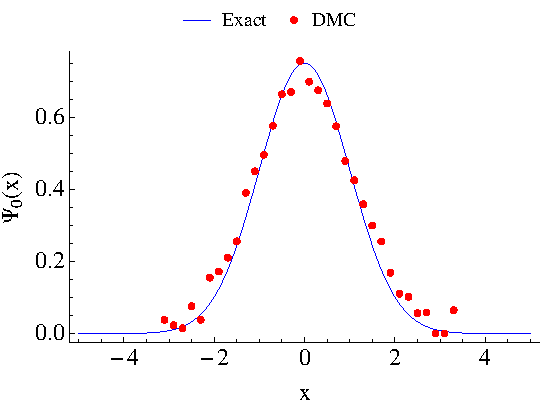
\includegraphics[width=0.5\textwidth]{notexact}
    \caption{DMC results for 1-d harmonic oscillator. Number of initial walkers was 10000, time step was 0.01, and number of time steps was 500. The exact energy is $E=\frac{1}{2}\hbar\omega$ and the DMC energy was $E=0.49\hbar\omega$.}
    \label{fig:1dho}
\end{figure}
I also did a calculation for a particle in a potential $V(x)=\frac{1}{2}x^4$, using the exact solution for the harmonic oscillator as the trial wave function. The DMC energy for this calculation was $E=0.57\hbar\omega$, and the resulting ground state wave function is shown in figure~\ref{fig:1dho4}.
\begin{figure}[h!]
  \centering
    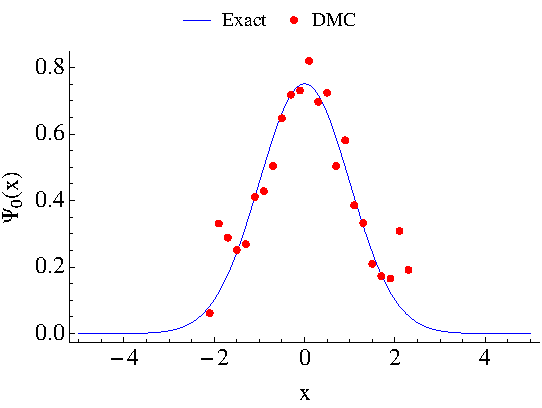
\includegraphics[width=0.5\textwidth]{notexact4}
    \caption{DMC results for particle in an $x^4$ potential. Number of initial walkers was 1000, time step was 0.01, and number of time steps was 500. The DMC energy was $E=0.57\hbar\omega$. The exact solution in this case represents the exact solution for the quantum harmonic oscillator.}
    \label{fig:1dho4}
\end{figure}


\section*{Auxiliary Field Diffusion Monte Carlo}
The methods described above are adequate for describing spin-independent potentials, but as described in \cite{schmidt1999} the number of spin-isospin states is 
\begin{equation}
  \frac{A!}{Z!(A-Z)!}2^A,
\end{equation}
where $A$ is the nucleons and $Z$ is the number of protons, which is exponential in the number of particles. The number of states to be sampled quickly becomes large. The AFDMC method is then used to simplify these methods.

My goal is to improve the trial function used in the current version of the code and so my comments will be directed toward this goal. The simplest trial wave function you can have is a slater determinant, which is the determinant of all of the single particle orbitals.
\begin{equation}
  \Psi_T(\mathbf{r}) \doteq \left| \\
  \begin{array}{cccc}
    \phi_1(\mathbf{r_1}) & \phi_2(\mathbf{r_1})  & \cdots & \phi_N(\mathbf{r_1})  \\
    \phi_1(\mathbf{r_2})  & \phi_2(\mathbf{r_2})  & \cdots & \phi_N(\mathbf{r_2})  \\
    \vdots & \vdots & \ddots & \vdots \\
    \phi_1(\mathbf{r_N})  & \phi_2(\mathbf{r_N})  & \cdots & \phi_N(\mathbf{r_N})  
  \end{array} \right|
\end{equation} 
This trial wave function does not include correlations. Ideally correlations would be included as
\begin{equation}
  \left<\mathrm{RS}\middle|\Psi_T\right> = \left<\mathrm{RS}\right| \prod\limits_{i<j}\left[f_c(r_{ij})\left[1+\sum\limits_{i<j,p}u_{ij}^p\mathcal{O}_{ij}^p\right]\right] \left|\Phi\right>,
  \label{equ:corrfull}
\end{equation}
where the sum on $p$ in our code goes from $1$ to $6$, where the first 6 $\mathcal{O}_{ij}^p$ are $1$, $\mathbf{\sigma}_i \cdot \mathbf{\sigma}_j$, $3\mathbf{\sigma}_i \cdot \hat{r}_{ij}\mathbf{\sigma}_j \cdot \hat{r}_{ij} - \mathbf{\sigma}_i \cdot \mathbf{\sigma}_j$, and the same things multiplied by $\mathbf{\tau}_i \cdot \mathbf{\tau}_j$. However, this requires too many operations. As discussed in \cite{gandolfi2014} the correlations have currently been included as
\begin{equation}
  \left<\mathrm{RS}\middle|\Psi_T\right> = \left<\mathrm{RS}\right| \left[\prod\limits_{i<j}f_c(r_{ij})\right]\left[1+\sum\limits_{i<j,p}u_{ij}^p\mathcal{O}_{ij}^p\right] \left|\Phi\right>.
  \label{equ:corrsimp}
\end{equation}
This is a first approximation and does not include many terms in the interaction. The next step to move from equation~\ref{equ:corrsimp} to equation~\ref{equ:corrfull} is to add the independent pair terms. This would look like
\begin{equation}
  \left<\mathrm{RS}\middle|\Psi_T\right> = \left<\mathrm{RS}\right| \left[\prod\limits_{i<j}f_c(r_{ij})\right]\left[1+\sum\limits_{i<j,p}u_{ij}^p\mathcal{O}_{ij}^p + \sum\limits_{i<j,p}\sum\limits_{k<l,p}u_{ij}^p\mathcal{O}_{ij}^pu_{kl}^p\mathcal{O}_{kl}^p\right] \left|\Phi\right>. 
\end{equation}
I am currently working on understanding the code so that I can add these extra terms into the trial wave function.

Even though my project does not deal with the sampling of the spin states I will mention the idea here for completeness. As discussed in \cite{schmidt1999} the non-central part of the potential can be written in the form
\begin{equation}
  V_\mathrm{nc} = \frac{1}{2} \sum\limits_{n=1}^{3N}(O_n^{(\sigma)})^2\lambda_n^{(\sigma)} + \frac{1}{2} \sum\limits_{\alpha=1}^{3} \sum\limits_{n=1}^{3N}(O_{n\alpha}^{(\sigma\tau)})^2\lambda_n^{(\sigma\tau)} + \frac{1}{2} \sum\limits_{\alpha=1}^{3} \sum\limits_{n=1}^{N}(O_{n\alpha}^{(\tau)})^2\lambda_n^{(\tau)},
\end{equation}
where the three squared operators are given by
\begin{equation}
  \begin{split}
    O_n^{(\sigma)} &= \sum\limits_i \boldsymbol{\sigma}_i \cdot \boldsymbol{\psi}_n^{(\tau)}(i) \\
    O_{n\alpha}^{(\sigma\tau)} &= \sum\limits_i \tau_{i\alpha} \boldsymbol{\sigma}_i \cdot \boldsymbol{\psi}_n^{(\sigma\tau)}(i) \\
    O_{n\alpha}^{(\tau)} &= \sum\limits_i \tau_{i\alpha} \psi_n^{(\tau)}(i),
  \end{split}
\end{equation}
where the $\psi$'s are the eigenfunctions of symmetric matrices that consist of phenomenological data. At this point the Hubbard-Stratonovich transformation can be used to take these squared operators and convert them to linear operators using the equation
\begin{equation}
  e^{-\frac{1}{2}\lambda_n O_n^2\Delta t} = \left( \frac{\Delta t |\lambda_n|}{2\pi} \right)^{1/2} \int\limits_{-\infty}^{\infty} dx e^{-\frac{1}{2}\Delta t |\lambda_n|x^2 - \Delta t s \lambda_n O_n x}.
\end{equation}
Notice how the $O_n$ term goes from quadratic to linear. This transformation is what gives the method the name Auxiliary Field.


\section*{Conclusion}
I conclusion, I have learned how to implement VMC and DMC methods and have applied these methods to the quantum harmonic oscillator as well as a similar $x^4$ potential. The ground state energies and wave functions that I obtained were close to the exact solutions for the harmonic oscillator. I have also learned the basics of the AFDMC method and have being working on understanding the existing code. Further work will include the addition of the extra terms in the trial wave function correlations. These additions will then be compared to the existing code for a variety of nuclear systems.


\bibliographystyle{unsrt} % unsrt shows in order of citations
\bibliography{references.bib}

\end{document}
